\section{Ergonomische Verbesserungen}

Dieser Teil wird sich auf die Implementierung einiger Lösungen für das im Abschnitt \ref{sec:analyse-ergo} erwähnte Problem konzentrieren.
Diese Lösungen basieren hauptsächlich auf den Eigenschaften der Angular-Frameworks, die im Abschnitt \ref{sec:angular} beschrieben wurden.

\subsection{animierte Illustrationen}

Eine interessante Herausforderung war die Erstellung von animierten Illustrationen, die eine sympathischere Schnittstellenbildung ermöglichten.
Dazu wurden Angular-Komponenten entwickelt, die aus \ac{SVG}-Vorlagen mit \ac{CSS}-Stilen und -Animationen bestehen, um bestimmte Bereiche des \ac{SVG} zu animieren.
Die SVGs wurden mit der Figma-Software so erstellt, dass einige Teile der endgültigen SVGs eine eindeutige \ac{HTML}-ID mithilfe der Syntax \lstinline{id="identifer"} haben.

\begin{lstlisting}[
  language=html,
  caption={Vereinfachtes SVG der Illustration der Seite 404 (siehe Abbildung \ref{fig:app_404_new})},
  captionpos=b,
  label={lst:wifi_illustration_svg}
]
<svg xmlns="http://www.w3.org/2000/svg" width="906" height="1006" viewBox="0 0 906 1006" fill="none">
  <g id="404">
    <g id="wifi">
      <path id="wave-3" d="M651.095 135.65C578.316 109.161 ..."/>
      <path id="wave-2" d="M613.188 239.798C579.397 227.499 ..."/>
      <path id="wave-1" d="M576.311 341.191C596.659 348.597 ..."/>
    </g>
    ...
\end{lstlisting}

\begin{lstlisting}[
  language=css,
  caption={Vereinfachter \ac{SASS}-Code, um das WIFI-Logo wie eine Welle zu animieren, die in der \ac{SVG} \ref{lst:wifi_illustration_svg} enthalten ist},
  captionpos=b
]
#wifi {
  [id^=wave] {
    animation: signal-wave 2s infinite;
  }

  #wave {
    &-2 { animation-delay: .2s; }
    &-3 { animation-delay: .4s; }
  }
}

@keyframes signal-wave {
  0% { opacity: 0; }
  60% { opacity: 1; }
  100% { opacity: 0; }
}
\end{lstlisting}

Insgesamt wurden 4 animierte Illustrationen erstellt, die über einen externen Link zum Service JSFiddle zugänglich sind.

\begin{table}[H]
  \begin{tabular}{p{0.5\linewidth} | p{0.5\linewidth}}
    Name der Komponente                                 & Link zur Vorschau                                                                               \\ \hline\hline

    \textbf{app-animated-illustration-peacefull-forest} & \href{https://jsfiddle.net/johannchopin/Lwu0nvm3/}{https://jsfiddle.net/johannchopin/Lwu0nvm3/} \\\hline
    \textbf{app-animated-illustration-404}              & \href{https://jsfiddle.net/johannchopin/puj3es5q/}{https://jsfiddle.net/johannchopin/puj3es5q/} \\\hline
    \textbf{app-animated-illustration-access-denied}    & \href{https://jsfiddle.net/johannchopin/pgkh0rfL/}{https://jsfiddle.net/johannchopin/pgkh0rfL/} \\\hline
    \textbf{app-animated-illustration-site-not-found}   & \href{https://jsfiddle.net/johannchopin/30js2zpr/}{https://jsfiddle.net/johannchopin/30js2zpr/}
  \end{tabular}
  \caption{Aktionen, die der Nutzer im Rahmen von Usability-Tests durchführen muss}
\end{table}

Diese Illustrationen können dann leicht in andere Seiten-Templates integriert werden:

\begin{lstlisting}[
  language=html,
  caption={Integration einer animierten Illustration bei einer falschen Eingabe der \textit{Site}-ID durch den Benutzer},
  captionpos=b
]
<div *ngIf="invalidSiteId">
  <app-animated-illustration-site-not-found></app-animated-illustration-site-not-found>
  <h2 class="bold">Site Not Found</h2>
  <p class="text-center">
    The site you're looking for might be removed or might never exist on earth.
  </p>
  ...
</div>
\end{lstlisting}


\subsection{Service für blinkende Favicons}

Die Animation des Favicons der Anwendung wird mithilfe eines Angular Service verwaltet, damit es von allen Komponenten der Anwendung konsumiert werden kann.
Dazu werden die beiden Favicons \textit{default.icon} und \textit{danger.ico} im Ordner \textit{src/assets/favicons} gespeichert.
Der \textit{assets}-Ordner in einem Angular-Projekt wird von der Rückgabe so bedient, dass Sie einfach auf die Favicons in der Anwendung zugreifen können, indem Sie den URI \textit{/favicons/default.ico} verwenden.
Der benutzerdefinierte Dienst \lstinline{FaviconService} wird den Dienst \lstinline{NgxFaviconService} verwenden, um einfach den Favicon-Link der Anwendung mithilfe seiner \lstinline{setCustomFavicon}-Methode zu bearbeiten.

Dieser verfügt über eine \lstinline{blink}-Methode, mit der zwei Favicons, die als Parameter übergeben werden, mithilfe eines JavaScript-Timers setInterval\footnote{Siehe \href{https://developer.mozilla.org/en-US/docs/Web/API/setInterval}{https://developer.mozilla.org/en-US/docs/Web/API/setInterval}} abwechseln können.
Die Methode \lstinline{stopBlink} stoppt diesen Timer.

\begin{lstlisting}[
  language=javascript,
  caption={Implementierung und Verwendung der \lstinline{blink}-Methode des Service \lstinline{FaviconService}},
  captionpos=b
]
private stopBlink(): void {
  clearInterval(this.blinkInterval)
}

private blink(faviconA: Favicons, faviconB: Favicons): void {
  this.blinkInterval = setInterval(() => {
    const faviconToShow = this.favicon === faviconA ? faviconB : faviconA
    this.set(faviconToShow)
  }, this.BLINK_INTERVAL)
}

public setDanger(blink = true): void {
  if (blink)
    this.blink(this.favicon, Favicons.DANGER)
  else
    this.set(Favicons.DANGER)
}
\end{lstlisting}

Der Service verbindet sich über ein Observable mit dem Brandmeldekanal und ruft die Methode lstinline{setDanger} auf, sobald ein Brand auftritt:

\begin{lstlisting}[
  language=javascript,
  caption={Methode, die sich mit den Alert Observables verbindet und die Anzeige von Favicons steuert},
  captionpos=b
]
private initFireWatcher = (): void => {
  this.subscription.add(this.oss
    .fireAlerts$()
    .subscribe((fireAlerts: Map<string, UpMessage[]>) => {
      const isFireDetected = fireAlerts.size > 0
      if (isFireDetected) this.setDanger()
      else this.setDefault()
    }))
}
\end{lstlisting}

\begin{figure}[H]
  \centering
  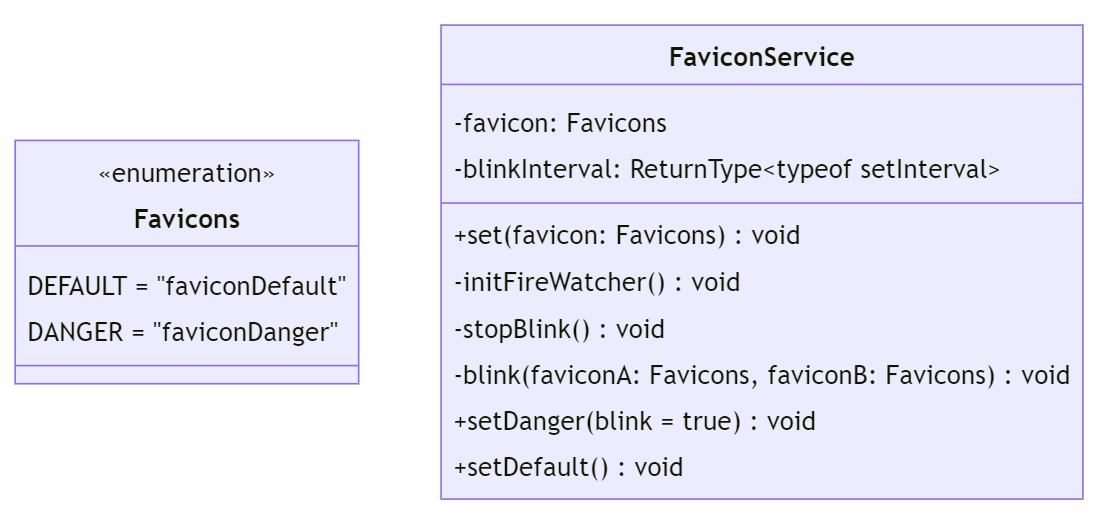
\includegraphics[width=10cm]{class_diagramm_favicon_service}
  \caption{Klassendiagramm für den Service \lstinline{FaviconService}}
  \label{fig:class_diagramm_favicon_service}
\end{figure}

\subsection{Pipe zur Lokalisierung von Distanzen}

Der Benutzer muss in der Lage sein, auszuwählen, in welchem metrischen Format er die Entfernungen auf seiner Benutzeroberfläche sehen möchte.
Die Anwendung wird einen Standardwert zwischen metrisch und imperial zuweisen, den der Benutzer auf einer Einstellungsseite unter \lstinline{/me/settings} ändern kann.

Genau wie im Abschnitt \ref{sec:consistent_interface} erwähnt, erzwingt ein Mangel an Zeit und Ressourcen die Datenspeicherung auf der Clientseite über den \lstinline{localstorage}.
Der bereits bestehende Service \lstinline{UserService} wird dafür zuständig sein, die Benutzereinstellungen zu initialisieren, zu speichern und wieder auszugeben.

\subsubsection{Speicherung und Wiedergabe von Daten}

\lstinline{UserService} wird die Benutzereinstellungen in einem JavaScript-Objekt speichern, das derzeit nur aus einer \lstinline{unitSystem}-Eigenschaft besteht.
Er speichert dieses Objekt unverändert als Zeichenkette, die er mithilfe der Methode \lstinline{JSON.stringify} generiert und mithilfe der Methode \lstinline{JSON.parse} parst.

\begin{lstlisting}[
  language=javascript,
  caption={Methode von \lstinline{UserService}, die das Lesen und Speichern der Benutzereinstellungen im \lstinline{localStorage} ermöglicht},
  captionpos=b
]
setLocalSettings = (settings: Partial<UserSettings>): void => {
  localStorage.setItem(UserService.SETTINGS_KEY, JSON.stringify({
    ...DEFAULT_SETTINGS,
    ...settings
  }))
}

getStoredSettings = (): string | null => {
  return localStorage.getItem(UserService.SETTINGS_KEY)
}

getLocalSettings = (): UserSettings => {
  const storedSettings = this.getStoredSettings()

  if (storedSettings) {
    try {
      return JSON.parse(storedSettings)
    } catch (error) {
      this.setLocalSettings(DEFAULT_SETTINGS)
      return DEFAULT_SETTINGS
    }
  }
  return DEFAULT_SETTINGS
}
\end{lstlisting}

\subsubsection{Festlegung der Standardauswahl}

Leider kann der Browser in seiner jetzigen Form nicht mit JavaScript erkennen, welche Art von Messung der Benutzer verwendet.
Eine naive Lösung, die aber bei den meisten Dryad-Kunden funktionieren wird, ist die Erkennung der Browsersprache, wie im Abschnitt \ref{sec:conceptionLocale} beschrieben.

Benutzer mit der Browsersprache \textit{en-US} oder \textit{en-GB} haben eine hohe Wahrscheinlichkeit, dass sie das imperiale System verwenden.
Alle anderen werden das metrische System als Standard verwenden.

\begin{lstlisting}[
  language=javascript,
  caption={Methode, die die Standardmaßeinheit abhängig von der Browsersprache festlegt},
  captionpos=b
]
getDefaultSettings = (): UserSettings => {
  const preferedLanguage = navigator.language
  const settings: UserSettings = {...DEFAULT_SETTINGS}

  if (preferedLanguage === 'en-US' || preferedLanguage === 'en-GB') {
    settings.unitSystem = "imperial"
  }

  return settings
}
\end{lstlisting}

Natürlich ist diese Technik der Standardbestimmung hypothetisch und erfordert, dass der Benutzer die Möglichkeit hat, diese Präferenz schnell zu ändern, was auf der Seite Settings der Fall ist.

\subsubsection{Umrechnung von metrischem zu imperialem System}

Jede Entfernung der Dryads-Systeme wird in der Einheit Meter gespeichert.
Es genügt also, eine Custom Pipe \lstinline{DistancePipe} zu erstellen, die als Parameter eine Entfernung in Metern annimmt und mithilfe des Service \lstinline{UserService} einen Wert im bevorzugten System des Benutzers zurückgibt.
Dieser muss auch die Größenordnung der Anfangsdistanz berücksichtigen, um einen relevanten Wert anzuzeigen, wie in der Tabelle \ref{table:metric_order_magnitude} näher erläutert.

Die vollständige Implementierung der \lstinline{DistancePipe} kann im Appendix \ref{lst:distancePipe} eingesehen werden.

\subsection{Bedingte Anzeige von Seitenabschnitten}

Die Anzeige der Sensorplanungsschnittstelle, wie sie im Abschnitt \ref{sec:conception_tunnel} beschrieben wurde, erfolgte schnell mit der Verwaltung von drei dynamischen Variablen, die den drei in \ref{fig:planing_v2_state_diagram} dargestellten Bedingungen entsprachen, und der Verwendung von Angular \lstinline{ng-template}\footnote{Siehe \href{https://angular.io/api/core/ng-template}{https://angular.io/api/core/ng-template}} und \lstinline{ng-container}\footnote{Siehe \href{https://angular.io/api/core/ng-container}{https://angular.io/api/core/ng-container}}.

\begin{lstlisting}[
  language=html,
  caption={Verwendung von Containers und Templates, die die Isolierung von Schnittstellenelementen und deren bedingtes Rendering ermöglichen.},
  captionpos=b
]
<ng-container *ngIf="addDeviceFlowStarted; else addDeviceButton">
  <p-dropdown
    [options]="deviceTypes"
    optionLabel="name"
    required="true"
    placeholder="Choose device type"
  ></p-dropdown>
  ...
</ng-container>

<ng-template #addDeviceButton>
  <button (click)="addDeviceFlowStarted = true">Add devices to packets</button>
</ng-template>
\end{lstlisting}
